%************************************************
\chapter{Modelling hippocampal place cells for visual localization}\label{ch:chapter5} % 
%************************************************


%%%%%%%%% BODY TEXT
\section{Introduction}

In the present work we study the hypothesis of the existence of a mechanism to mimic place cells from appearance information in order to provide localization within an indoor context. In other words, our research question could be enunciated as ``given a series of images, is there a way we can generate a place cell response that can be used to localize a subject with respect to previously visited places?''.

The topic of biologically inspired visual localization has not been explored to the extent of visual localization on its own. To the best of our knowledge, Milford and colleagues have extensively studied the matter, remarkably setting a seminal precedent with the publication of RatSLAM \cite{milford2004ratslam}, a persistent navigation and mapping model based on the hippocampus of rodents that continuously performed SLAM while simultaneously interacting with other navigation systems, such as odometry and landmark detection. Their recent work has been focused on taking RatSLAM to larger scales and incorporating more complex visual landmark detection models. However, we believe those vision models do not capture all the information bandwidth that is required in the same proportion by our brains to provide localization.

\subsection{Summary of contributions}

Our approach to indoor localization is novel for several reasons. In first place, we use those appearance-based methods that, among others, best mimic the biological visual sensory inputs. In second place, we contribute a model for appearance-based localization based on hippocampal place cells mimicry that is able to encode distinctive information from unseen queries based on the recall of previously visited places. In third place, we provide a complete pipeline of visual localization by incorporating a decoder of the place cell localization model in the form of a generalized neural network (GNN). Finally, we provide an evaluation of the method by testing the system with a publicly available database of indoor sequences of more than 120,000 frames and 3 km of length. We demonstrate that an achievable error of less than X m is possible. Finally, we provide a discussion on the potential advantages and pitfalls of this type of localization system.



\section{Biological background}

Navigation is one of the most complex tasks performed by animals, as it involves integration of multiple sensory inputs, requires combined processing with past information (memory) and the execution of physical actions to perform navigation movements.

John O'Keefe, together with Edvard and May-Britt Moser, received the Nobel Prize in Physiology or Medicine for their discovery of the place and grid cells in the brain, respectively. This award highlights the importance of the discovery, let alone because these cells are located in one of the least known but more attractive areas of our brains: the hippocampus, with a key role in memory, and its adjacent areas.

Humans, like other animals, need a sense of position to perform basic interaction with the environment. This interaction is often finding our way from one place to another and place awareness is integrated with distance and direction information to navigate.

Early findings in the topic suggested that a cognitive map of the environment with a set of landmarks is created and that spatial relationships between them are used to navigate \cite{keefe1978hippocampus}. It was the pioneering ability of O'Keefe and colleagues to carry out experiments to record nerve cells firing rates in moving animals that it was found that these maps originate in the hippocampus and surrounding areas.

\subsection{Place cells}


Place cells are a special type of neurons located in the hippocampus which fire when an animal ``recognises'' a particular place in the environment. Grid cells, located next to the hippocampus in the entorhinal cortex, provides the brain with a reference system for navigation, a ``grid'' that is used as a form of coordinates for the creation of spatial maps. The combination of place and grid cells neural circuitry is crucial for the execution of navigation tasks.

The area in the environment at which the place cells show intense firing patterns is called place field. The combination of multiple place fields yields a spatial map of the environment, and multiple spatial maps formed by combination of different place cell activity patterns -- with repetition -- are thought to be stored in the hippocampus. It is the unique combination of a specific number of place cell firing patterns in a specific order what gives place to a unique environment representation \cite{okeefe1971hippocampus}.

It was when studying the entorhinal cortex looking for similar place coding cells when the Mosers discovered the grid cell type, with unprecedented properties \cite{hafting2005microstructure}. Specially, they present multiple-locations firing pattern with hexagonal shape, thought to be part of a navigation or path integration system with distance measuring and coordinate system properties. Apart from grid cells, there are other cells in the entorhinal cortex that have a spatial function. These are head direction cells, which act similarly to a compass; border cells, active in reference to boundaries; and combined cells. The Mosers demonstrated that all these cells project to the hippocampus, concretely to the CA1 area where place cells are located \cite{zhang2013optogenetic}. This corroborates the studies that show that entorhinal cortex cells that encode spatial information, specially	 border cells, play a role in the firing activity of place cells \cite{bush2014grid}.

\subsection{Appearance-based methods as models of sensory inputs to place cell models}

\subsubsection{Gradient operators as V1 receptive field models}

In \cite{bush2014grid}, Bush et al. establish the idea that grid cells and place cells are not successive links of a chain when performing localization and navigation tasks, but complementary and interconnected processing units to encode spatial maps. Importantly, they claim that place cell spatial firing is determined by sensory inputs, among which vision plays a major role.

This motivated us to create models of place cell encoding patterns from elements of the computer vision research that modelled visual cortex representation. An exceptional case is the one of gradient operations, present in SIFT and SIFT-like descriptors, as models of the pyramidal neurons in the primary visual cortex (V1), which exhibit strong direction selectivity, spatial phase invariance and response inhibition \cite{hubel1962receptive, dhruv2014cascaded,carandini2006simple}.

The seminal work of Hubel and Wiesel \cite{hubel1962receptive} proposed that the response of V1 neurons is produced by stimuly of higher complexity than ganglion cells in the retina and the lateral geniculate nucleus (LGN). In particular, it is known that simple and complex cells in the V1 display orientation selectivity produced by bars or edge stimuli \cite{payne2001cat}.

This orientation selective simple cells can be modelled as the output of a 2D Gabor function \cite{daugman1985uncertainty}, and through tuning their parameters, different combinations of orientation and phase can be achieved. In particular, the steerability of the Gabor filter can represent the orientation selectivity of these neurons, whilst the phase parameter of the filter can be viewed as their shape selectivity. 

We have therefore studied the use of 2D Gabor-like filters, which have been used for a great variety of applications in Computer Vision, from action recognition \cite{shu2014bio} to face recognition \cite{liao2013partial} and appearance-based indoor localization \cite{rivera2015appearance}, and often as part of a biologically inspired system \cite{shu2014bio}. Mathematically, the over-completeness of Gabor outputs, i.e. multiple Gabor output values to a single pixel, provides advantageous invariance properties for descriptors computed on local image patches. In particular, the main benefit of using Gabor filters resides in the combination of symmetric and antisymmetric responses that yields a description of local regions in an image that are either phase selective or phase invariant. The real part of these filters presents the simple cell receptive fields behavior described above \cite{jones1987evaluation}. In Fig. \ref{fig:simple_cell} we illustrate the orientation selectivity of V1 simple cell receptive fields, and an example 2D Gabor fit spatial and 2D views.


\begin{figure}[h]
\centering
\includegraphics[width=.8\textwidth]{./gfx/Chapter05//simple_cell_gabor.pdf}
\caption{Orientation sensitive simple cells which only respond to a bar of certain size and orientation.}
\label{fig:simple_cell}
\end{figure}

Also relevant to this study, the difference of Gaussians (DoG) space representation found in the scale invariant feature transform (SIFT) keypoint detection \cite{lowe2004distinctive} may be seen as an approximation of the spatial receptive field of a retinal ganglion cell. Lowe also suggested that the process behind the computation of the orientation of the frequencies is similar to the behavior of complex cells in V1. In particular, each bin of the histogram of oriented gradients (HOG) can be seen as a single orientation-selective neuron.

We have seen that we can use 2D Gabor like features as a biologically plausible input to place cells models to provide localization. Though differently inspired, we also used SIFT in order to constitute a baseline for our experiments.

\subsubsection{BOVW model spatial binning as a form of population encoding}

Here we need to include the notions of the spatial binning achieved during clustering as a form of population encoding: close locations in space correspond to close positions in V1 receptive fields. Expand.

\section{Overview of the system}

Here I have added a draft of the pipeline only for training. I need to talk about the testing (decoding too).


\subsection{System Pipeline}

\begin{figure}[h]
\centering
\includegraphics[width=\linewidth]{./gfx/Chapter05//nn_pipeline.pdf}
\caption{Overview of the training pipeline. The diagram of the neural network is merely illustrative, it does not represent the real architecture used.}
\label{fig:pipeline}
\end{figure}

\subsection{Data}

\section{Modelling a single place cell: the tuning curve encoder}

We refer to place cells, according to the previous section, as a biological term to denominate a special type of neurons sensitive to specific spatial locations. This point forward, the term ``place cell'' will also be used not only to describe a biological entity but to refer to the output of a series of algorithms that mimic the behaviour of their biological counterparts.

Given the nature of image matching techniques, one would expect high scores when two images are visually similar, and low ones when they are dissimilar. 

%Additionally, as the visual paths datasets analysed in this work present a sequential

If we take an unseen query frame from one of the passes of the RSM dataset and use one of the similarty metrics described in Section \ref{sec:metrics}

\section{Decoding location representations: a neural network approach}


\section{Experiments}

\subsection{Hippocampal modelling experiments}

\subsection{Localization experiments}

\section{Results}

\begin{figure}
	\centering
	\setlength\figureheight{0.3\textwidth}
	\setlength\figurewidth{0.4\textwidth}
		% This file was created by matlab2tikz.
% Minimal pgfplots version: 1.3
%
%The latest updates can be retrieved from
%  http://www.mathworks.com/matlabcentral/fileexchange/22022-matlab2tikz
%where you can also make suggestions and rate matlab2tikz.
%
\definecolor{mycolor1}{rgb}{0.00000,0.44700,0.74100}%
\definecolor{mycolor2}{rgb}{0.85000,0.32500,0.09800}%

%
\begin{tikzpicture}

\begin{axis}[%
width=0.95092\figurewidth,
height=\figureheight,
at={(0\figurewidth,0\figureheight)},
scale only axis,
xmin=517,
xmax=816,
xlabel={Frame index},
ymin=1.79650837845272,
ymax=7.47640317281087,
ylabel={$\chi{}^\text{2}\text{ score}$}
]
\addplot [color=mycolor2,solid,line width=2.0pt,forget plot]
  table[row sep=crcr]{%
517	5.45564129617479\\
518	5.28480574819777\\
519	5.38022258546617\\
520	5.04640165964762\\
521	4.91818147235447\\
522	5.02140005429586\\
523	4.9060054090288\\
524	5.14407377772861\\
525	4.78613996505737\\
526	4.74626959694756\\
527	4.60538254843818\\
528	4.73193724950155\\
529	4.89160471492344\\
530	4.61402278476291\\
531	4.74068803257412\\
532	4.82834929890103\\
533	4.78515206442939\\
534	5.00995551215278\\
535	4.93059447076586\\
536	4.747631099489\\
537	4.85051237212287\\
538	4.85323116514418\\
539	4.79317005475362\\
540	4.78844994968838\\
541	4.7296888033549\\
542	4.57528159353468\\
543	4.6541080739763\\
544	4.73621863789029\\
545	4.60128768285116\\
546	4.72721687952677\\
547	4.7022082540724\\
548	4.51559209823608\\
549	4.45021396213108\\
550	4.61597768465678\\
551	4.58577950795492\\
552	4.56056160397\\
553	4.61316866344876\\
554	4.44940259721544\\
555	4.33124679989285\\
556	4.31974034839206\\
557	4.24667429924011\\
558	4.18328481250339\\
559	4.32105019357469\\
560	4.36144169171651\\
561	4.33154243893093\\
562	4.2965227233039\\
563	4.45881326993306\\
564	4.60404780175951\\
565	4.9832649230957\\
566	5.21849367353651\\
567	5.42206896675958\\
568	5.61464606391059\\
569	5.32002242406209\\
570	5.31870725419786\\
571	5.20021793577406\\
572	5.55876763661702\\
573	5.52424425548977\\
574	5.40127817789714\\
575	5.50023322635227\\
576	5.73416566848755\\
577	5.55387417475383\\
578	5.5627646446228\\
579	5.47471041149563\\
580	5.35248724619548\\
581	4.86793337927924\\
582	4.91971654362149\\
583	4.92856052186754\\
584	5.1939090622796\\
585	4.77915970484416\\
586	4.61318797535366\\
587	4.59124125374688\\
588	4.83357630835639\\
589	4.78117969301012\\
590	4.8751319249471\\
591	5.01082160737779\\
592	5.23354652192858\\
593	4.6385703086853\\
594	4.53041002485487\\
595	4.51224210527208\\
596	4.43363348642985\\
597	4.25946267445882\\
598	4.22609305381775\\
599	4.34774973657396\\
600	4.57303765085008\\
601	4.32682673136393\\
602	4.77783237563239\\
603	4.9052480061849\\
604	4.89262798097399\\
605	4.71505321396722\\
606	4.99992277887132\\
607	4.91769223743015\\
608	4.94722530576918\\
609	5.03998618655735\\
610	4.98740741941664\\
611	5.11870463689168\\
612	5.16300662358602\\
613	5.19595686594645\\
614	5.05345845222473\\
615	4.81346085336473\\
616	4.98365359836155\\
617	5.10461118486193\\
618	5.3875585132175\\
619	5.45500458611382\\
620	5.10809373855591\\
621	5.40080017513699\\
622	5.12411006291707\\
623	5.11253976821899\\
624	5.29478883743286\\
625	5.38006231519911\\
626	5.26761012607151\\
627	5.07983054055108\\
628	4.79844037691752\\
629	4.7360757721795\\
630	4.55040812492371\\
631	4.55683490965101\\
632	4.32798796229892\\
633	4.38316342565748\\
634	4.57085434595744\\
635	4.71197700500488\\
636	5.20676475101047\\
637	5.29618379804823\\
638	5.53390868504842\\
639	5.37041934331258\\
640	5.56473557154338\\
641	5.70307895872328\\
642	5.30179659525553\\
643	5.38066954082913\\
644	5.54609791437785\\
645	5.42192618052165\\
646	5.84239138497247\\
647	5.49786647160848\\
648	5.54475773705377\\
649	5.51714981926812\\
650	5.45711406071981\\
651	5.44256104363336\\
652	5.12285571628147\\
653	5.11807007259793\\
654	5.33797539605035\\
655	5.66756502787272\\
656	5.50892194112142\\
657	5.86675696902805\\
658	5.8700491587321\\
659	5.71904346677992\\
660	5.90887721379598\\
661	6.13676097657945\\
662	6.19742769665188\\
663	6.42192517386542\\
664	6.30267741945055\\
665	6.34279457728068\\
666	6.27500221464369\\
667	6.28113868501451\\
668	6.38645627763536\\
669	6.43902895185682\\
670	6.78609715567695\\
671	6.9065891901652\\
672	6.71403990851508\\
673	6.70098299450344\\
674	6.66558986239963\\
675	6.7139032681783\\
676	6.78372716903687\\
677	6.76429753833347\\
678	7.00557661056519\\
679	6.82014653417799\\
680	7.00547329584758\\
681	7.34336815940009\\
682	7.20823060141669\\
683	6.99682813220554\\
684	7.24651824103461\\
685	7.23865800433689\\
686	7.34053574668037\\
687	7.34751473532783\\
688	7.37640317281087\\
689	7.37493318981594\\
690	7.32039319144355\\
691	7.26464568244086\\
692	7.08425818549262\\
693	6.96295788553026\\
694	6.90606005986532\\
695	7.08241897159153\\
696	6.66772707303365\\
697	6.62142117818197\\
698	6.64435042275323\\
699	6.69112764464484\\
700	6.59604427549574\\
701	6.51153024037679\\
702	6.47479195064968\\
703	6.78648434744941\\
704	6.22314156426324\\
705	5.96851372718811\\
706	6.07606569925944\\
707	6.0125810570187\\
708	6.13718112309774\\
709	6.05301419893901\\
710	5.86252167489794\\
711	5.8945533964369\\
712	5.94143915176392\\
713	5.79714462492201\\
714	5.77606577343411\\
715	5.80971254242791\\
716	5.595112880071\\
717	5.6970772213406\\
718	5.93423128128052\\
719	5.84677373038398\\
720	5.82072750727336\\
721	5.70003567801581\\
722	5.5985779232449\\
723	5.41437101364136\\
724	5.41969439718458\\
725	5.26762652397156\\
726	5.31281068589952\\
727	5.33975100517273\\
728	5.22491206063165\\
729	5.03604883617825\\
730	5.22387671470642\\
731	5.00555160310533\\
732	4.94978168275621\\
733	4.51597449514601\\
734	4.7652227083842\\
735	4.92013684908549\\
736	4.85085704591539\\
737	4.84549196561178\\
738	4.6559042930603\\
739	4.86927668253581\\
740	4.71941457854377\\
741	4.81414641274346\\
742	4.79970055156284\\
743	4.69480657577515\\
744	4.71684855884976\\
745	4.59916199578179\\
746	4.60451703601413\\
747	4.55340411927965\\
748	4.76788369814555\\
749	4.70615172386169\\
750	4.6492067972819\\
751	4.7372952832116\\
752	4.70831603474087\\
753	4.95494400130378\\
754	4.93097477489048\\
755	5.05009076330397\\
756	4.83696320321825\\
757	4.65081408288744\\
758	4.9603201813168\\
759	5.27593053711785\\
760	5.34850931167603\\
761	5.34796449873182\\
762	5.31409517923991\\
763	5.15496057934231\\
764	5.20180945926242\\
765	5.18936035368178\\
766	4.8254066573249\\
767	5.08930932150947\\
768	4.86718906296624\\
769	4.62061770757039\\
770	4.98884542783101\\
771	5.15281282530891\\
772	5.03079618348016\\
773	4.79297688272264\\
774	4.88556533389621\\
775	5.0670190387302\\
776	4.6277256541782\\
777	4.46976200739543\\
778	4.50152950816684\\
779	4.35459629694621\\
780	4.15776922967699\\
781	4.18754514058431\\
782	4.16014623641968\\
783	4.23905968666077\\
784	4.11976922882928\\
785	3.84921227561103\\
786	4.09121913380093\\
787	4.26308623949687\\
788	3.93736775716146\\
789	4.12939588228862\\
790	4.14773575464884\\
791	4.02434510654873\\
792	3.93602151340908\\
793	3.89979214138455\\
794	3.81887470351325\\
795	3.75678775045607\\
796	3.81119052569071\\
797	3.97538926866319\\
798	3.73644529448615\\
799	3.62051859166887\\
800	3.63900767432319\\
801	3.4945670498742\\
802	3.44758110576206\\
803	3.41365891032749\\
804	3.53506263097127\\
805	3.68221312099033\\
806	3.50561817487081\\
807	3.18562004301283\\
808	2.92959801355998\\
809	2.77806928422716\\
810	2.53599411911435\\
811	2.5533709526062\\
812	2.44258156087663\\
813	2.23334169387817\\
814	1.9372197786967\\
815	1.97369148996141\\
816	1.79650837845272\\
};


\addplot [color=mycolor1,solid,line width=2.0pt,forget plot]
  table[row sep=crcr]{%
517	5.45564129617479\\
518	5.37355654327958\\
519	5.21705055236816\\
520	5.14466546073792\\
521	5.10476355199461\\
522	5.02677491939429\\
523	4.99369739059709\\
524	4.95151845967328\\
525	4.93448695637821\\
526	4.9382541179657\\
527	4.9249986529981\\
528	4.91614664925469\\
529	4.90358046743605\\
530	4.88218153160786\\
531	4.86746233359151\\
532	4.85760750992751\\
533	4.83489814751879\\
534	4.82152560173519\\
535	4.80884125211217\\
536	4.78737886475022\\
537	4.76278513104612\\
538	4.73903547392951\\
539	4.7215891002137\\
540	4.70695415963518\\
541	4.71049302505528\\
542	4.7056532776545\\
543	4.70845456782923\\
544	4.71323872045054\\
545	4.71882281768349\\
546	4.72699681323131\\
547	4.73064615775128\\
548	4.74396783586532\\
549	4.75172641704412\\
550	4.76428025812248\\
551	4.77966727096748\\
552	4.80270366117257\\
553	4.8194778841369\\
554	4.83317502555933\\
555	4.85074007916613\\
556	4.8632257774033\\
557	4.86403361577836\\
558	4.86677982963942\\
559	4.86511870738871\\
560	4.87049247456246\\
561	4.87113591548807\\
562	4.86629256045197\\
563	4.86094582756631\\
564	4.86177044498677\\
565	4.8616220724015\\
566	4.86459029937277\\
567	4.87347887108385\\
568	4.88530414553186\\
569	4.88331132248686\\
570	4.88186483967061\\
571	4.8774775993797\\
572	4.87199648167271\\
573	4.86676935057521\\
574	4.86219545448719\\
575	4.85672141473039\\
576	4.85646137683029\\
577	4.85169127738935\\
578	4.85505176131147\\
579	4.86435472884146\\
580	4.87581148763903\\
581	4.88387909714056\\
582	4.89925151509222\\
583	4.91423942172338\\
584	4.92701850564572\\
585	4.9408663524792\\
586	4.95425135208095\\
587	4.97103057480723\\
588	4.98540186773893\\
589	4.99748164455907\\
590	4.9989141655617\\
591	4.99064818963983\\
592	4.98170093722354\\
593	4.97129206214092\\
594	4.9726703496747\\
595	4.97545192787707\\
596	4.97357184221955\\
597	4.97034801647506\\
598	4.96218201254501\\
599	4.95628939193933\\
600	4.95209664930832\\
601	4.94487005026162\\
602	4.93902792681912\\
603	4.92917212877684\\
604	4.91537069949974\\
605	4.90279087349941\\
606	4.89631076626767\\
607	4.88890501863562\\
608	4.87664843578728\\
609	4.86010260646846\\
610	4.85585147669526\\
611	4.85786757934121\\
612	4.87042928336699\\
613	4.87987025254438\\
614	4.89523206870842\\
615	4.90533997520568\\
616	4.9166443418213\\
617	4.92622663644977\\
618	4.93976186678793\\
619	4.95711410180782\\
620	4.97821319995283\\
621	4.99838243860777\\
622	5.03068710616927\\
623	5.05664166571602\\
624	5.08107040041969\\
625	5.10033799569353\\
626	5.12340508404773\\
627	5.13697097523142\\
628	5.14141194890686\\
629	5.14601280791959\\
630	5.15872550551313\\
631	5.17235085753356\\
632	5.1844167698538\\
633	5.2031827221652\\
634	5.22012278282183\\
635	5.2350541307272\\
636	5.25118010168443\\
637	5.27105263950062\\
638	5.2914908197191\\
639	5.31941871199748\\
640	5.34981088681556\\
641	5.37754845781391\\
642	5.40143398903395\\
643	5.41967031907062\\
644	5.43867953726494\\
645	5.46584148039353\\
646	5.49411284734332\\
647	5.5304899723892\\
648	5.56317364872178\\
649	5.59187148866199\\
650	5.61810674472731\\
651	5.64762293130092\\
652	5.68239633188226\\
653	5.72251586578871\\
654	5.76883220942923\\
655	5.81515340145483\\
656	5.86512561341802\\
657	5.92666398478744\\
658	5.98431841694579\\
659	6.03382808605289\\
660	6.08555341740044\\
661	6.127020626652\\
662	6.16874209499143\\
663	6.20575446336448\\
664	6.24669290886444\\
665	6.28363571740062\\
666	6.31664213031328\\
667	6.35670027494971\\
668	6.39146739014693\\
669	6.42038289976228\\
670	6.4506713462795\\
671	6.4759780317207\\
672	6.49985273787224\\
673	6.52182546116057\\
674	6.54482955510925\\
675	6.57001350580159\\
676	6.59355397992123\\
677	6.62189427633134\\
678	6.64958247792424\\
679	6.67914388509565\\
680	6.69048218175668\\
681	6.69986160596212\\
682	6.70413321270153\\
683	6.70704202695228\\
684	6.71557544850979\\
685	6.71851701963516\\
686	6.71292029919268\\
687	6.70673919102502\\
688	6.69693335383928\\
689	6.68661635803257\\
690	6.67505046407652\\
691	6.66555475648028\\
692	6.65155422984878\\
693	6.63748526951623\\
694	6.62718327623916\\
695	6.60801341041686\\
696	6.58585296790886\\
697	6.56515900402112\\
698	6.54266094134238\\
699	6.51712586279629\\
700	6.49071343685764\\
701	6.45977260736652\\
702	6.4301504267046\\
703	6.39615398577822\\
704	6.36359818019564\\
705	6.32340584428403\\
706	6.2801509168413\\
707	6.2351982842227\\
708	6.19342182607067\\
709	6.13769644350151\\
710	6.08721817215554\\
711	6.03782227628626\\
712	5.98687007854315\\
713	5.93521882941664\\
714	5.87972844376856\\
715	5.82970565787248\\
716	5.77776216595622\\
717	5.73143335426746\\
718	5.68728524541098\\
719	5.64215762328669\\
720	5.59388067608788\\
721	5.55166506226641\\
722	5.51050375324258\\
723	5.4678313797023\\
724	5.42858150324313\\
725	5.3900122674955\\
726	5.35200566661601\\
727	5.31654655095401\\
728	5.27413495273547\\
729	5.24825336981793\\
730	5.22707910548532\\
731	5.20614084148623\\
732	5.18214864038826\\
733	5.15181461915948\\
734	5.12951474124882\\
735	5.11754349353903\\
736	5.10639973670717\\
737	5.09428800909427\\
738	5.08442985714158\\
739	5.07175424093562\\
740	5.0593480555649\\
741	5.05106739176103\\
742	5.03327819657704\\
743	5.01603489127559\\
744	4.99604336745074\\
745	4.97155133072211\\
746	4.95703724398364\\
747	4.94793999708699\\
748	4.9401119393286\\
749	4.92732178597223\\
750	4.91952461882784\\
751	4.91450846276316\\
752	4.89997733315102\\
753	4.88456610757477\\
754	4.87365754986025\\
755	4.85591713317127\\
756	4.8386154520809\\
757	4.82305960428147\\
758	4.81579780308297\\
759	4.80505978223148\\
760	4.78872574916502\\
761	4.76828401915881\\
762	4.75289069606063\\
763	4.74487400108995\\
764	4.72585545159251\\
765	4.71381425370975\\
766	4.70021403619762\\
767	4.68439045568713\\
768	4.66890504625108\\
769	4.65223042548649\\
770	4.63630619503203\\
771	4.61900559736758\\
772	4.60385838117189\\
773	4.58768502546816\\
774	4.56789509833805\\
775	4.54690146148881\\
776	4.52448742865435\\
777	4.49971704120809\\
778	4.46895453313581\\
779	4.43798890324677\\
780	4.40706996177059\\
781	4.38350363356186\\
782	4.36013228850029\\
783	4.32391391833083\\
784	4.27602958111536\\
785	4.22357162137151\\
786	4.16618447076707\\
787	4.10984316001944\\
788	4.0544884861732\\
789	3.99390751136944\\
790	3.92753729555342\\
791	3.86933902683171\\
792	3.80213900758566\\
793	3.76206392768427\\
794	3.70389658551157\\
795	3.64771100655391\\
796	3.58290216851687\\
797	3.533371826862\\
798	3.48501014709473\\
799	3.44571603063553\\
800	3.400025913611\\
801	3.36231850466848\\
802	3.30612304384224\\
803	3.25225202340648\\
804	3.1855489508311\\
805	3.12186565721668\\
806	3.05844036485783\\
807	2.97056146671897\\
808	2.88727670479444\\
809	2.79667528382054\\
810	2.69914532624758\\
811	2.53378304447791\\
812	2.35337503015259\\
813	2.21038685336946\\
814	2.07666858037313\\
815	1.90247321570361\\
816	1.79650837845272\\
};

\end{axis}
\end{tikzpicture}%

	\caption{Single tuning curve with and without smoothing}
\end{figure}

\subsection{Features of a place cell}

\begin{figure}
\centering
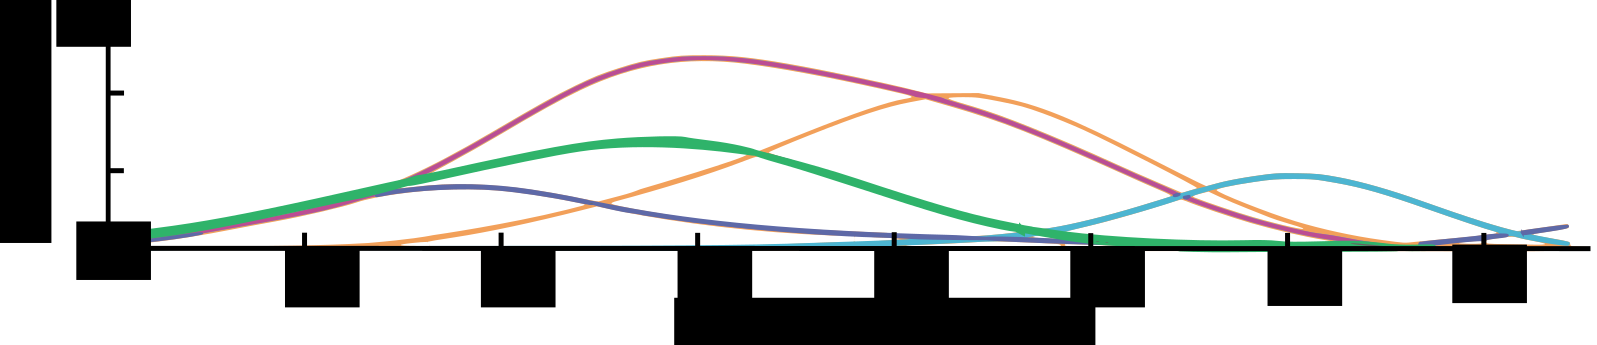
\includegraphics[width=\linewidth]{./gfx/Chapter05//dragoi_et_al_place_cell.png}
\caption{Caption}
\label{}
\end{figure}

\subsection{Modelling a place field}

\begin{figure}
	\centering
	\setlength\figureheight{0.3\textwidth}
	\setlength\figurewidth{0.8\textwidth}
		% This file was created by matlab2tikz.
% Minimal pgfplots version: 1.3
%
%The latest updates can be retrieved from
%  http://www.mathworks.com/matlabcentral/fileexchange/22022-matlab2tikz
%where you can also make suggestions and rate matlab2tikz.
%
\definecolor{mycolor1}{rgb}{0.00000,0.44700,0.74100}%
%
\begin{tikzpicture}

\begin{axis}[%
width=\figurewidth,
height=\figureheight,
at={(0\figurewidth,0\figureheight)},
scale only axis,
xmin=0,
xmax=200,
xlabel={Distance covered by place field (cm)},
ymin=6,
ymax=16,
ylabel={$\chi{}^\text{2}\text{ score}$},
axis x line*=bottom,
axis y line*=left,
legend style={at={(0.01,1), font=\footnotesize, pos=north west},anchor=north west,legend cell align=left,align=left,draw=white!15!black}
]
\addplot [color=mycolor1,solid,forget plot]
  table[row sep=crcr]{%
1	7.68376493453979\\
2	8.06428162256877\\
3	8.17457895278931\\
4	8.26771565846034\\
5	8.39854224522909\\
6	8.48510087620128\\
7	8.56682128172654\\
8	8.59774649937948\\
9	8.59330785975737\\
10	8.59233688053332\\
11	8.65034806100946\\
12	8.6829998618678\\
13	8.70982235356381\\
14	8.73964701200786\\
15	8.76372538114849\\
16	8.81391369669061\\
17	8.84981777793482\\
18	8.88881823891087\\
19	8.92264235647101\\
20	8.92992637031957\\
21	8.96761618162456\\
22	8.98679191187808\\
23	8.9777606662951\\
24	8.99128396887528\\
25	9.02349341543097\\
26	9.06194029356304\\
27	9.07705984617534\\
28	9.08789730072021\\
29	9.16552889974494\\
30	9.20696765498111\\
31	9.28507794831928\\
32	9.33594211779143\\
33	9.40688434400056\\
34	9.47275663677015\\
35	9.51096138201262\\
36	9.57157029603657\\
37	9.59795033304315\\
38	9.63532538163035\\
39	9.68495173203318\\
40	9.73211971082185\\
41	9.76160094612523\\
42	9.84171430688155\\
43	9.87884355846204\\
44	9.91074536976061\\
45	9.97806167602539\\
46	10.0605657477128\\
47	10.1543830068488\\
48	10.1903820037842\\
49	10.1771721087004\\
50	10.2039889285439\\
51	10.2577184375964\\
52	10.2896445424933\\
53	10.3242208581222\\
54	10.3520846617849\\
55	10.3246375134117\\
56	10.327644799885\\
57	10.2831729085822\\
58	10.2989949176186\\
59	10.3075340672543\\
60	10.3240774054276\\
61	10.3239422346416\\
62	10.338483057524\\
63	10.355751087791\\
64	10.3346134988885\\
65	10.3087987397846\\
66	10.2878237272564\\
67	10.2445729406256\\
68	10.3025695399234\\
69	10.307963521857\\
70	10.3145902031346\\
71	10.3082494233784\\
72	10.2968946256136\\
73	10.29000347539\\
74	10.3067134556017\\
75	10.3624493950292\\
76	10.4283245990151\\
77	10.473633465014\\
78	10.4986793618453\\
79	10.5597394140143\\
80	10.5885658766094\\
81	10.6724687877454\\
82	10.7098674272236\\
83	10.7820806001362\\
84	10.8456166417975\\
85	10.9124588213469\\
86	10.9945609946\\
87	11.0395386344508\\
88	11.0759984066612\\
89	11.0878075549477\\
90	11.174538913526\\
91	11.2535098226447\\
92	11.2934483477944\\
93	11.4110110433478\\
94	11.4771789249621\\
95	11.5847304494757\\
96	11.6558806770726\\
97	11.6956441778886\\
98	11.741151106985\\
99	11.8461348884984\\
100	11.9315716090955\\
101	12.0584896991127\\
102	12.1596005088405\\
103	12.2862813849198\\
104	12.3939189910889\\
105	12.5373618477269\\
106	12.6995426479139\\
107	12.8576787647448\\
108	13.0239966543097\\
109	13.1540311512194\\
110	13.319268678364\\
111	13.5711681968287\\
112	13.7674868232325\\
113	13.9117409555536\\
114	14.1342613822535\\
115	14.3111799641659\\
116	14.5127577028776\\
117	14.7724789569252\\
118	14.9731010637785\\
119	15.1494964800383\\
120	15.3023914537932\\
121	15.4148659455149\\
122	15.5046606565777\\
123	15.5718047493383\\
124	15.6386499906841\\
125	15.6548606972945\\
126	15.6602967914782\\
127	15.6785095616391\\
128	15.6893093711451\\
129	15.6443962799875\\
130	15.5395172520688\\
131	15.4437499297293\\
132	15.3918147338064\\
133	15.2391425684879\\
134	15.160818150169\\
135	15.0714185112401\\
136	14.8675742902254\\
137	14.6906490827862\\
138	14.4995145295796\\
139	14.317297433552\\
140	14.1889972686768\\
141	14.0079520878039\\
142	13.8699980284038\\
143	13.7053286903783\\
144	13.5121448416459\\
145	13.346944156446\\
146	13.1712456251446\\
147	12.9792186335513\\
148	12.7931142104299\\
149	12.6321003562526\\
150	12.4593344738609\\
151	12.2989568208393\\
152	12.1092826943649\\
153	11.8975028489765\\
154	11.7115875043367\\
155	11.5410103045012\\
156	11.3823467555799\\
157	11.2529855025442\\
158	11.1149904351485\\
159	10.9747475071957\\
160	10.8977248543187\\
161	10.7714399538542\\
162	10.6372470855713\\
163	10.5698853040996\\
164	10.4631252288818\\
165	10.3797384563245\\
166	10.3210554122925\\
167	10.2368787464343\\
168	10.1455332605462\\
169	10.0590010693199\\
170	9.96171790675113\\
171	9.92465465947201\\
172	9.85105524565044\\
173	9.83175578870271\\
174	9.82826910520854\\
175	9.82929244794344\\
176	9.80742454528808\\
177	9.77649437753778\\
178	9.74254201587878\\
179	9.71514656669215\\
180	9.70644775189851\\
181	9.70242635827315\\
182	9.68256599024722\\
183	9.67866546229312\\
184	9.65845037761487\\
185	9.62630086196096\\
186	9.63348855470356\\
187	9.62079033098723\\
188	9.57925399981047\\
189	9.54161443208393\\
190	9.48096516257838\\
191	9.46174189918919\\
192	9.39641958124497\\
193	9.28440195719401\\
194	9.22090192941519\\
195	9.10513149608265\\
196	9.0278107325236\\
197	8.91698932647705\\
198	8.69013175964355\\
199	8.5991382598877\\
200	8.65595436096191\\
};
\addplot [color=mycolor1,solid,forget plot]
  table[row sep=crcr]{%
1	7.78974533081055\\
2	8.24546146392822\\
3	8.2059232711792\\
4	8.30384009225028\\
5	8.46911366780599\\
6	8.57545757293701\\
7	8.66584014892578\\
8	8.72392470041911\\
9	8.77890508315143\\
10	8.76167397750051\\
11	8.81231232693321\\
12	8.84206525902999\\
13	8.89677614914743\\
14	8.95330574637965\\
15	9.03483245247289\\
16	9.11082383206016\\
17	9.16337766145405\\
18	9.21636787213777\\
19	9.25363314779181\\
20	9.32508639285439\\
21	9.37708774365877\\
22	9.41500633641293\\
23	9.44026716131913\\
24	9.4964888723273\\
25	9.51564066033614\\
26	9.57845276280453\\
27	9.61700093118768\\
28	9.67566058510228\\
29	9.76951488695647\\
30	9.84211876517848\\
31	9.88287117606715\\
32	9.90614042784038\\
33	9.95397221414666\\
34	9.94960664447985\\
35	9.94154001537122\\
36	9.93845397547671\\
37	9.93972999171207\\
38	9.94791593049702\\
39	9.91885471343994\\
40	9.86866258320056\\
41	9.8816738630596\\
42	9.86880212081106\\
43	9.85691512258429\\
44	9.86012709768195\\
45	9.86251314062821\\
46	9.85767108515689\\
47	9.86313167371248\\
48	9.88262693505538\\
49	9.85518069016306\\
50	9.86689171038176\\
51	9.85894594694439\\
52	9.86834626448782\\
53	9.87308411849172\\
54	9.89184304287559\\
55	9.88775579552901\\
56	9.86541582408704\\
57	9.83238124847412\\
58	9.82683628483822\\
59	9.85457169382196\\
60	9.84547620070608\\
61	9.87177146108527\\
62	9.89337198357833\\
63	9.93357327109889\\
64	9.95364560578999\\
65	9.97571071825529\\
66	9.97774068932784\\
67	9.96628911871659\\
68	9.99899798945377\\
69	10.0420335468493\\
70	10.0874010889154\\
71	10.1202272114001\\
72	10.1565657163921\\
73	10.1864740974025\\
74	10.2600338082564\\
75	10.3353486312063\\
76	10.4312352130288\\
77	10.5360646498831\\
78	10.6370698025352\\
79	10.700949769271\\
80	10.7748168644152\\
81	10.8565941358867\\
82	10.9276397604691\\
83	10.9812740024767\\
84	11.0603665301674\\
85	11.1463016710783\\
86	11.2400730534604\\
87	11.329712365803\\
88	11.3847010763068\\
89	11.4552882847033\\
90	11.5636912898013\\
91	11.6875077799747\\
92	11.7985651116622\\
93	11.9058998007523\\
94	12.0099947578029\\
95	12.1207789872822\\
96	12.2099598332455\\
97	12.2552975102475\\
98	12.3610138140227\\
99	12.4899568557739\\
100	12.5691422914204\\
101	12.6803599407798\\
102	12.8016963757967\\
103	12.9322004318237\\
104	13.0519447828594\\
105	13.206052077444\\
106	13.3588140387284\\
107	13.5333973734002\\
108	13.7005219710501\\
109	13.8285800532291\\
110	13.9563547937494\\
111	14.0349952798141\\
112	14.1013716647499\\
113	14.1864039772435\\
114	14.2109204342491\\
115	14.2269237919858\\
116	14.266135567113\\
117	14.2827341180099\\
118	14.2736311460796\\
119	14.2758127011751\\
120	14.2420792830618\\
121	14.1923249897204\\
122	14.1247635389629\\
123	14.0710356360988\\
124	14.0194581684313\\
125	13.9296033758866\\
126	13.7861822529843\\
127	13.6250945141441\\
128	13.453824444821\\
129	13.2667096288581\\
130	13.1250362898174\\
131	12.9663466403359\\
132	12.781004554347\\
133	12.6344159276862\\
134	12.5241462807906\\
135	12.4098825454712\\
136	12.2475808294196\\
137	12.0535706469887\\
138	11.9036610251979\\
139	11.7468564384862\\
140	11.6221565447356\\
141	11.4624991667898\\
142	11.3056739004035\\
143	11.1152617805882\\
144	10.9251345082333\\
145	10.801794052124\\
146	10.7027071902626\\
147	10.6084232832256\\
148	10.4968896665071\\
149	10.384888799567\\
150	10.3036232496563\\
151	10.1993318356966\\
152	10.0996779893574\\
153	9.97909385279605\\
154	9.85852597889147\\
155	9.79813359913073\\
156	9.75442550056859\\
157	9.69155070656224\\
158	9.65326334300794\\
159	9.57966924968519\\
160	9.53380233363101\\
161	9.46464528535542\\
162	9.39612448842902\\
163	9.35308556807668\\
164	9.2422446702656\\
165	9.15449970646909\\
166	9.07869484550075\\
167	9.00080003236469\\
168	8.93617208380448\\
169	8.86870073017321\\
170	8.81002882907265\\
171	8.78196811676025\\
172	8.70360577733893\\
173	8.70128056877538\\
174	8.66400911933497\\
175	8.63318400633963\\
176	8.57585036127191\\
177	8.4945794908624\\
178	8.42566879172074\\
179	8.37487855710481\\
180	8.34225682208413\\
181	8.29535717713205\\
182	8.24076075302927\\
183	8.23479767849571\\
184	8.21042311818976\\
185	8.18993523246363\\
186	8.14898566195839\\
187	8.12949215738397\\
188	8.07790214137027\\
189	8.04920269313611\\
190	7.97547782094855\\
191	7.95771581248233\\
192	7.86952066421509\\
193	7.80752712885539\\
194	7.78445606965285\\
195	7.68587064743042\\
196	7.65943537818061\\
197	7.55697100503104\\
198	7.4216682434082\\
199	7.29020881652832\\
200	7.29163646697998\\
};
\addplot [color=mycolor1,solid,forget plot]
  table[row sep=crcr]{%
1	7.53792572021484\\
2	8.41769440968831\\
3	8.45193405151367\\
4	8.43963091714042\\
5	8.55593861473931\\
6	8.53339498693293\\
7	8.54694087688739\\
8	8.57917029062907\\
9	8.58090967290542\\
10	8.57476480383622\\
11	8.62809542605751\\
12	8.60669537594444\\
13	8.6144303271645\\
14	8.62445846356844\\
15	8.65019406770405\\
16	8.7224756542005\\
17	8.74752566688939\\
18	8.77536562869423\\
19	8.8014474166067\\
20	8.82829796640496\\
21	8.87733755613628\\
22	8.91618071104351\\
23	8.92337106403552\\
24	8.92923324986508\\
25	8.9604031412225\\
26	9.0033947794061\\
27	9.0177785471866\\
28	9.05181879746287\\
29	9.13538962916324\\
30	9.19506057940031\\
31	9.31139609688207\\
32	9.3479780899851\\
33	9.44872951507568\\
34	9.52539358640972\\
35	9.56304394571405\\
36	9.64082431793213\\
37	9.68633932816355\\
38	9.76453324368125\\
39	9.84450330232319\\
40	9.91436526649877\\
41	9.97219191099468\\
42	10.07719366174\\
43	10.1646941335578\\
44	10.2257384250039\\
45	10.2896133724012\\
46	10.3917447642276\\
47	10.4897841905293\\
48	10.5431990372507\\
49	10.5694021927683\\
50	10.6057810532419\\
51	10.6896443617971\\
52	10.7062985269647\\
53	10.7471121737832\\
54	10.770522017228\\
55	10.765433261269\\
56	10.768040205303\\
57	10.7172088121113\\
58	10.7385144484671\\
59	10.7417746594078\\
60	10.7527739876195\\
61	10.7460303055613\\
62	10.7402690586291\\
63	10.7531814575195\\
64	10.7657255875437\\
65	10.7440102225856\\
66	10.7015496806095\\
67	10.6753126445569\\
68	10.7077682896664\\
69	10.6848265999242\\
70	10.6560910877429\\
71	10.6374908246492\\
72	10.6371201966938\\
73	10.6588354110718\\
74	10.6684704830772\\
75	10.6907630217703\\
76	10.7655312889501\\
77	10.7710518084074\\
78	10.8048191070557\\
79	10.8590187273527\\
80	10.8969832972476\\
81	10.9915351365742\\
82	11.035874467147\\
83	11.0843456669858\\
84	11.1650513598793\\
85	11.2362122284739\\
86	11.2843780517578\\
87	11.3392468502647\\
88	11.4264742198743\\
89	11.4989445334987\\
90	11.6320958890413\\
91	11.7259882374814\\
92	11.8274932158621\\
93	11.9552382418984\\
94	12.053123072574\\
95	12.1462819952714\\
96	12.2421918166311\\
97	12.3172590356124\\
98	12.3936640086927\\
99	12.4854025087859\\
100	12.534016107258\\
101	12.6280541169016\\
102	12.7412469261571\\
103	12.8599204515156\\
104	12.9735060240093\\
105	13.1089091551931\\
106	13.2714973248933\\
107	13.3795740729884\\
108	13.4991196582192\\
109	13.6079698361849\\
110	13.7665105116995\\
111	13.9488102762323\\
112	14.0583223543669\\
113	14.1919745896992\\
114	14.3112695091649\\
115	14.4063755838495\\
116	14.4961554878636\\
117	14.5627100091231\\
118	14.6310757586831\\
119	14.6866511294716\\
120	14.7194541629992\\
121	14.7554474880821\\
122	14.734463239971\\
123	14.7125848970915\\
124	14.713884654798\\
125	14.6313302391454\\
126	14.5577580803319\\
127	14.4838040502448\\
128	14.3606536764848\\
129	14.1767507352327\\
130	13.9540864542911\\
131	13.7614224584479\\
132	13.5786791851646\\
133	13.3998501426295\\
134	13.2691153978047\\
135	13.1527816872848\\
136	13.0029961937352\\
137	12.8520841598511\\
138	12.6930209210044\\
139	12.5574824684545\\
140	12.4233148976376\\
141	12.2672917717382\\
142	12.1529839666266\\
143	12.0049771258706\\
144	11.8650938335218\\
145	11.7438351982518\\
146	11.6200240787707\\
147	11.4794015382466\\
148	11.3773241545025\\
149	11.278971270511\\
150	11.2159019269441\\
151	11.1297710318314\\
152	11.0236329530415\\
153	10.920069292972\\
154	10.7903712925158\\
155	10.6970327778866\\
156	10.6029547641152\\
157	10.5435114910728\\
158	10.4690053337499\\
159	10.3816188009162\\
160	10.3227086318167\\
161	10.2236641331723\\
162	10.1257185183073\\
163	10.0536445818449\\
164	9.95836252915232\\
165	9.88172621476023\\
166	9.82479893533807\\
167	9.74290541598671\\
168	9.65706197839034\\
169	9.57831091629831\\
170	9.50285986850136\\
171	9.46935648667185\\
172	9.42649675670423\\
173	9.39508282510858\\
174	9.37478396767064\\
175	9.35160902926796\\
176	9.30778377934506\\
177	9.25709302801835\\
178	9.18979996129086\\
179	9.1447222358302\\
180	9.12176332975689\\
181	9.10318354556435\\
182	9.09480471360056\\
183	9.11250797070955\\
184	9.09981747677452\\
185	9.07572073685495\\
186	9.069841033534\\
187	9.06011596478914\\
188	9.01991979699386\\
189	9.00630720038163\\
190	8.92895452599776\\
191	8.85897443169042\\
192	8.80698408800013\\
193	8.73993463516235\\
194	8.69839209776658\\
195	8.64068339087746\\
196	8.54771746529473\\
197	8.3624597958156\\
198	8.20139741897583\\
199	8.11229467391968\\
200	7.99361085891724\\
};
\addplot [color=mycolor1,solid,forget plot]
  table[row sep=crcr]{%
1	7.67510747909546\\
2	8.02797969182332\\
3	8.02783708572388\\
4	8.08701481137957\\
5	8.24081150690714\\
6	8.29345785487782\\
7	8.36440977683434\\
8	8.41121021906535\\
9	8.43581460503971\\
10	8.43798685073853\\
11	8.4774785292776\\
12	8.49419905010023\\
13	8.52700665122584\\
14	8.56879816557232\\
15	8.60205730639006\\
16	8.68092797931872\\
17	8.7052482805754\\
18	8.73601767891332\\
19	8.77790717074745\\
20	8.79095519216437\\
21	8.81890477632221\\
22	8.82694154036672\\
23	8.78551287400095\\
24	8.78290151294909\\
25	8.81253854851973\\
26	8.82332284826981\\
27	8.81395013708817\\
28	8.83184949975264\\
29	8.89935262579667\\
30	8.92547175758763\\
31	9.01900191056101\\
32	9.05566225553814\\
33	9.12206047459652\\
34	9.19217606594688\\
35	9.20620817887156\\
36	9.2657806998805\\
37	9.3228255322105\\
38	9.37231339906391\\
39	9.434991334614\\
40	9.50735473632813\\
41	9.56483499627364\\
42	9.6824019582648\\
43	9.75151307959305\\
44	9.80388099268863\\
45	9.89888898949874\\
46	10.0026696857653\\
47	10.1136653297826\\
48	10.1646432374653\\
49	10.1941034919337\\
50	10.1848286076596\\
51	10.2266358325356\\
52	10.2565713179739\\
53	10.2984978525262\\
54	10.3494261189511\\
55	10.3442784359581\\
56	10.3306920904862\\
57	10.2721648467214\\
58	10.2919540907207\\
59	10.2862624620136\\
60	10.3010430586965\\
61	10.3115950634605\\
62	10.3090416757684\\
63	10.3365298823306\\
64	10.3042678833008\\
65	10.2822478444953\\
66	10.2208267011141\\
67	10.1734511726781\\
68	10.183015923751\\
69	10.1968219656693\\
70	10.1925565819991\\
71	10.1710378747237\\
72	10.1365072350753\\
73	10.1085773267244\\
74	10.1103923697221\\
75	10.1220025012368\\
76	10.1753087796663\\
77	10.1656276301334\\
78	10.1758953395643\\
79	10.1889085267719\\
80	10.2079265996029\\
81	10.260909030312\\
82	10.2833560642443\\
83	10.3270774138601\\
84	10.3511800765991\\
85	10.401598428425\\
86	10.4432211926109\\
87	10.5041371897647\\
88	10.5497394862928\\
89	10.6001655679\\
90	10.663481411181\\
91	10.7435932159424\\
92	10.8124535711188\\
93	10.931635806435\\
94	10.9691206781488\\
95	11.0290167959113\\
96	11.1110087444908\\
97	11.1623848864907\\
98	11.2283980218988\\
99	11.2915564587242\\
100	11.3453365125154\\
101	11.4001959750527\\
102	11.4921314841823\\
103	11.5784212413587\\
104	11.658107707375\\
105	11.7882344597264\\
106	11.8914904845388\\
107	11.9813881422344\\
108	12.1017289914583\\
109	12.2389668916401\\
110	12.354983078806\\
111	12.5136497899106\\
112	12.6622972488403\\
113	12.822884258471\\
114	12.9826191851967\\
115	13.1128613321405\\
116	13.2977402837653\\
117	13.5214897456922\\
118	13.6824388002094\\
119	13.8312137503373\\
120	14.0305517096269\\
121	14.2058560220819\\
122	14.4053375344527\\
123	14.5904177615517\\
124	14.7244217019332\\
125	14.8436335513466\\
126	14.949035744918\\
127	15.0006844369989\\
128	15.0161018371582\\
129	15.0288929186369\\
130	14.9910567936144\\
131	14.9285201022499\\
132	14.9096168216906\\
133	14.8343047091835\\
134	14.7732572555542\\
135	14.6616721404226\\
136	14.5128327419883\\
137	14.4135453073602\\
138	14.2835412778352\\
139	14.0880775953594\\
140	13.9174405148155\\
141	13.6847401669151\\
142	13.4714191838315\\
143	13.2680985802098\\
144	13.0545234680176\\
145	12.8781844691226\\
146	12.7126985851087\\
147	12.5381305594193\\
148	12.3527762262445\\
149	12.1949956793534\\
150	12.0266299498709\\
151	11.8459328099301\\
152	11.6811317644621\\
153	11.5529118086162\\
154	11.4084239758943\\
155	11.2576429969386\\
156	11.0978627455862\\
157	10.9945855391653\\
158	10.8922077480115\\
159	10.7812860890439\\
160	10.7249665511282\\
161	10.6217170012625\\
162	10.5288836328607\\
163	10.469824590181\\
164	10.3625089745773\\
165	10.2785511016846\\
166	10.1991938038876\\
167	10.1336879730225\\
168	10.058065063075\\
169	9.97604274749756\\
170	9.90472442225406\\
171	9.87831226148103\\
172	9.80503383435701\\
173	9.77287568544087\\
174	9.73923577760395\\
175	9.71639005761397\\
176	9.65735601124011\\
177	9.61607802541632\\
178	9.5541854155691\\
179	9.48004250777395\\
180	9.43491443834807\\
181	9.37427671332108\\
182	9.31643320384778\\
183	9.31158899006091\\
184	9.26490452415065\\
185	9.19263538561369\\
186	9.16806421781841\\
187	9.11777009462055\\
188	9.05044116471943\\
189	9.00928720675017\\
190	8.91300756052921\\
191	8.83908319473267\\
192	8.75723325504976\\
193	8.64322557449341\\
194	8.53571477303138\\
195	8.45154064351862\\
196	8.37836027145386\\
197	8.15532091685704\\
198	8.01396207809448\\
199	7.92976951599121\\
200	7.84953498840332\\
};
\addplot [color=mycolor1,solid,forget plot]
  table[row sep=crcr]{%
1	8.81433868408203\\
2	9.23034540812174\\
3	9.2335823059082\\
4	9.34099102020264\\
5	9.54948817359077\\
6	9.62183111364191\\
7	9.69446035531851\\
8	9.789870262146\\
9	9.89363743277157\\
10	9.90569335535953\\
11	9.97196067006964\\
12	9.97963669425563\\
13	10.011661529541\\
14	10.0828073903134\\
15	10.0923711375186\\
16	10.1208186902498\\
17	10.1297840821116\\
18	10.0884271420931\\
19	10.0830247276708\\
20	10.0356542687667\\
21	10.0244679701956\\
22	9.96340726551256\\
23	9.88462889821906\\
24	9.79272837387888\\
25	9.69513120149311\\
26	9.60526702278539\\
27	9.47716226075825\\
28	9.40247194390548\\
29	9.36437140013042\\
30	9.32312734503495\\
31	9.31482922403436\\
32	9.29491384405839\\
33	9.255506264536\\
34	9.23975286985699\\
35	9.20001024948923\\
36	9.19531992862099\\
37	9.19868820591977\\
38	9.18832949588173\\
39	9.17787366164358\\
40	9.18031562002082\\
41	9.23067338843095\\
42	9.26121651498895\\
43	9.31725110505757\\
44	9.3741387818989\\
45	9.44598679793508\\
46	9.51956362473337\\
47	9.59774308455618\\
48	9.66161175778037\\
49	9.68455525448448\\
50	9.70375176479942\\
51	9.7342277326082\\
52	9.75940854925859\\
53	9.80198147422389\\
54	9.83344906254819\\
55	9.84236375909103\\
56	9.84428867540861\\
57	9.84098861092015\\
58	9.90835104490581\\
59	9.94883276286878\\
60	9.96704392684133\\
61	10.0100489666587\\
62	10.0333815122906\\
63	10.0832332309924\\
64	10.1272608606439\\
65	10.1879708641454\\
66	10.2204498993723\\
67	10.2322383177908\\
68	10.2850543574283\\
69	10.3521736044633\\
70	10.4070605227822\\
71	10.4727369609632\\
72	10.5166173734163\\
73	10.571258946469\\
74	10.6429464440597\\
75	10.7131730631778\\
76	10.787567941766\\
77	10.8225504222669\\
78	10.8318123064543\\
79	10.8629351164165\\
80	10.8722321359735\\
81	10.9024934266743\\
82	10.8593071385434\\
83	10.7903524699964\\
84	10.7128779260736\\
85	10.635695658232\\
86	10.5806472176\\
87	10.5005375711541\\
88	10.3787698745728\\
89	10.2658300901714\\
90	10.1498509959171\\
91	10.0393358531751\\
92	9.94387466029117\\
93	9.86416922117534\\
94	9.73504995044909\\
95	9.61683930848774\\
96	9.51589870452881\\
97	9.38871474015085\\
98	9.28313195077996\\
99	9.2079385456286\\
100	9.11097185235274\\
101	9.07585209294369\\
102	9.03614340330425\\
103	9.0284598501105\\
104	8.99892350247032\\
105	8.98294619510048\\
106	8.9573887272885\\
107	8.94512808950324\\
108	8.9349933423494\\
109	8.95447540283203\\
110	8.98234849227102\\
111	8.96920846637926\\
112	8.95385897786994\\
113	8.98447267632735\\
114	9.03605330617804\\
115	9.04860948261462\\
116	9.10419574536775\\
117	9.15457238649067\\
118	9.17053463584498\\
119	9.15528111708792\\
120	9.14118345160233\\
121	9.17276101363333\\
122	9.16511520586516\\
123	9.20452082784552\\
124	9.23201761747661\\
125	9.24844962672183\\
126	9.27211635991146\\
127	9.29224651738217\\
128	9.27942542025917\\
129	9.26802188471744\\
130	9.24410975606818\\
131	9.20184803009033\\
132	9.16427486821225\\
133	9.12231349945068\\
134	9.09987258911133\\
135	9.0798965253328\\
136	9.00989597722104\\
137	8.98267068360981\\
138	8.96830162249113\\
139	8.94864037162379\\
140	8.92396429965371\\
141	8.87839196857653\\
142	8.82449737348055\\
143	8.78394744270726\\
144	8.76934367731998\\
145	8.77443464178788\\
146	8.76824007536236\\
147	8.78366736361855\\
148	8.78206473902652\\
149	8.81885357906944\\
150	8.85141638705605\\
151	8.85671987031636\\
152	8.83402864556563\\
153	8.81142776890805\\
154	8.78990123146459\\
155	8.80176047274941\\
156	8.82996017054508\\
157	8.87393273805317\\
158	8.9145359742014\\
159	8.92137878819516\\
160	8.95175943876568\\
161	8.96687392184609\\
162	8.94563228205631\\
163	8.93641632481625\\
164	8.87744993912546\\
165	8.85818059820878\\
166	8.83726702238384\\
167	8.81949515091745\\
168	8.80027073308041\\
169	8.7787937867014\\
170	8.78570190228914\\
171	8.8056899622867\\
172	8.83311602943822\\
173	8.88890427037289\\
174	8.94124723735609\\
175	8.94182882810894\\
176	8.93705433293393\\
177	8.90617345508776\\
178	8.87179771222566\\
179	8.83730070214522\\
180	8.80530879372045\\
181	8.78288540087248\\
182	8.74752398541099\\
183	8.76241104226363\\
184	8.71782837415996\\
185	8.63711357116699\\
186	8.56437853762978\\
187	8.47666785591527\\
188	8.40000383477462\\
189	8.33727294520328\\
190	8.25480779848601\\
191	8.16453499543039\\
192	8.00565217523014\\
193	7.8574714978536\\
194	7.74527736810538\\
195	7.64499633962458\\
196	7.56967035929362\\
197	7.41352272033691\\
198	7.36305418014526\\
199	7.42254781723022\\
200	7.2355489730835\\
};
\addplot [color=mycolor1,solid,forget plot]
  table[row sep=crcr]{%
1	8.98475742340088\\
2	9.55461184183756\\
3	9.53240470886231\\
4	9.57648658752441\\
5	9.7242743174235\\
6	9.7584753036499\\
7	9.83451850597675\\
8	9.95610637664795\\
9	10.0165695302627\\
10	10.0656920985172\\
11	10.1510985525031\\
12	10.1597460194638\\
13	10.1719956648977\\
14	10.2301388288799\\
15	10.2250874669928\\
16	10.2775150098299\\
17	10.2665961918078\\
18	10.2497899908769\\
19	10.2211738887586\\
20	10.1774712110821\\
21	10.1569156646728\\
22	10.1414686504163\\
23	10.0689720354582\\
24	10.0132412659494\\
25	9.91811968150892\\
26	9.84489179912366\\
27	9.7492497594733\\
28	9.68741687975432\\
29	9.62254569405003\\
30	9.5737439205772\\
31	9.52614553351151\\
32	9.49697358984696\\
33	9.43012659173263\\
34	9.42926582537199\\
35	9.33892591376054\\
36	9.32634182980186\\
37	9.28923591814543\\
38	9.26123639156944\\
39	9.24919374365556\\
40	9.24497298190468\\
41	9.20275120986135\\
42	9.21157365096243\\
43	9.19809597416928\\
44	9.18426257685611\\
45	9.19653280157792\\
46	9.20237445831299\\
47	9.23116538399144\\
48	9.22919057544909\\
49	9.17943076083534\\
50	9.16199282595986\\
51	9.14716800890471\\
52	9.14793150048507\\
53	9.12211091894853\\
54	9.12318043959768\\
55	9.09918554205644\\
56	9.08858936711362\\
57	9.03892276161595\\
58	9.04170026277241\\
59	9.04042143570749\\
60	9.01395928232293\\
61	8.99255536731921\\
62	8.98390875364605\\
63	9.01100575296502\\
64	9.02769560562937\\
65	9.07308387756347\\
66	9.05223434849789\\
67	9.0169015181692\\
68	9.0335774170725\\
69	9.05804719422993\\
70	9.07736441963597\\
71	9.09459324886924\\
72	9.10707990746749\\
73	9.11371592471474\\
74	9.12810541454114\\
75	9.1619045859889\\
76	9.16139191075375\\
77	9.13598401922929\\
78	9.09456248032419\\
79	9.11238258763363\\
80	9.07896578939337\\
81	9.05841556348299\\
82	8.98322572206196\\
83	8.89662815395154\\
84	8.80311667291742\\
85	8.73276431936967\\
86	8.70730999896401\\
87	8.67683277632061\\
88	8.57523401159989\\
89	8.49021713357223\\
90	8.39973005495573\\
91	8.30863513444599\\
92	8.241766151629\\
93	8.16711867483039\\
94	8.05332203915245\\
95	8.02664156963951\\
96	7.97653097855417\\
97	7.89314751876028\\
98	7.79993162657085\\
99	7.77381510483591\\
100	7.74067833549098\\
101	7.69534605427792\\
102	7.69744062423706\\
103	7.67728052641216\\
104	7.66290383589895\\
105	7.628720961119\\
106	7.59444756256907\\
107	7.59042308205052\\
108	7.56735141653764\\
109	7.54788609554893\\
110	7.5318344517758\\
111	7.50550250003212\\
112	7.5006278439572\\
113	7.51268469659906\\
114	7.50924117941605\\
115	7.50656137968365\\
116	7.53768905840422\\
117	7.58197751798128\\
118	7.56859056573165\\
119	7.52485777202406\\
120	7.52684992238095\\
121	7.50847206617656\\
122	7.51437992798655\\
123	7.48842997299997\\
124	7.49423383411608\\
125	7.46874101538407\\
126	7.464574387199\\
127	7.47445437782689\\
128	7.49382131978085\\
129	7.48716959200407\\
130	7.48115732795314\\
131	7.44880179355019\\
132	7.42068140130294\\
133	7.38428055612664\\
134	7.37390590968885\\
135	7.36619788721988\\
136	7.30497239765368\\
137	7.29953665482371\\
138	7.32007997914365\\
139	7.31930135425768\\
140	7.31691701788651\\
141	7.29283009077373\\
142	7.31085195039448\\
143	7.33399830366436\\
144	7.35898534875167\\
145	7.38055409883198\\
146	7.42059669996563\\
147	7.45729157799169\\
148	7.53057833721763\\
149	7.58716299659327\\
150	7.64852840022037\\
151	7.68990980951409\\
152	7.72256567603663\\
153	7.74290940636083\\
154	7.77241573835674\\
155	7.8391843093069\\
156	7.86363812496788\\
157	7.89441673379195\\
158	7.91414873223556\\
159	7.91859671944066\\
160	7.96103281723826\\
161	7.99145658392655\\
162	7.97460977654708\\
163	7.96528605410927\\
164	7.94347338927419\\
165	7.91868270070929\\
166	7.89341414602179\\
167	7.85660088689704\\
168	7.83156093798186\\
169	7.81390759819432\\
170	7.80023592396786\\
171	7.80904910438939\\
172	7.81358001106664\\
173	7.81381574429964\\
174	7.80923913654528\\
175	7.80214693671779\\
176	7.77584168785497\\
177	7.76324081420898\\
178	7.76260644511173\\
179	7.72831291901438\\
180	7.69645690917969\\
181	7.66744335074174\\
182	7.6419388620477\\
183	7.64288693980167\\
184	7.61853072517797\\
185	7.55219690423263\\
186	7.49924750077097\\
187	7.43407906984028\\
188	7.35321777745297\\
189	7.31555765553524\\
190	7.24448828948171\\
191	7.18311450355931\\
192	7.09887176401475\\
193	7.03073581059774\\
194	6.95335953052227\\
195	6.86017916419289\\
196	6.79278013441298\\
197	6.6300208909171\\
198	6.56814556121826\\
199	6.67524846394857\\
200	6.63803768157959\\
};
\addplot [color=mycolor1,solid,forget plot]
  table[row sep=crcr]{%
1	7.42668342590332\\
2	7.7494470278422\\
3	7.72162313461304\\
4	7.753860609872\\
5	7.98453108469645\\
6	8.05623340606689\\
7	8.18162536621094\\
8	8.28020699818929\\
9	8.37644554586971\\
10	8.41024860582854\\
11	8.47356224060059\\
12	8.5127753458525\\
13	8.56745034769962\\
14	8.6504588880037\\
15	8.70380133076718\\
16	8.80214314711721\\
17	8.86353502775493\\
18	8.89925213863975\\
19	8.91904002741764\\
20	8.96249655673378\\
21	9.03348752071983\\
22	9.06271553039551\\
23	9.03724544926694\\
24	9.05558244805587\\
25	9.04643294685765\\
26	9.09303645083779\\
27	9.05124724538703\\
28	9.0558096735101\\
29	9.11467055270546\\
30	9.17829724362022\\
31	9.24240890302156\\
32	9.29634320108514\\
33	9.36129298963045\\
34	9.44331972222579\\
35	9.47070814433851\\
36	9.53372217479505\\
37	9.58285030565764\\
38	9.6662046030948\\
39	9.71602053391306\\
40	9.76563895376105\\
41	9.82438845383493\\
42	9.90105463329114\\
43	9.93708500109221\\
44	9.98212016256232\\
45	10.027766729656\\
46	10.1259446395071\\
47	10.1925515124672\\
48	10.2528242813913\\
49	10.236942190873\\
50	10.2066971628289\\
51	10.2102881983707\\
52	10.1900674920333\\
53	10.1533951006438\\
54	10.1282542881213\\
55	10.0842015115838\\
56	10.0149131072195\\
57	9.8964436681647\\
58	9.83635239852102\\
59	9.79454959066291\\
60	9.72467547968814\\
61	9.6555575822529\\
62	9.60322114040977\\
63	9.57666994396009\\
64	9.5256986618042\\
65	9.45905755695544\\
66	9.40643109773335\\
67	9.30171785856548\\
68	9.26041101154528\\
69	9.24162844607704\\
70	9.18637697320235\\
71	9.15595626831055\\
72	9.1101050627859\\
73	9.06669451061048\\
74	9.03530778382954\\
75	9.0308646151894\\
76	9.02083572588469\\
77	8.9795927248503\\
78	8.90252625314813\\
79	8.8671612488596\\
80	8.83303055010344\\
81	8.81542712763736\\
82	8.78166118421052\\
83	8.71397364766974\\
84	8.64083410564222\\
85	8.57888793945312\\
86	8.56863358146266\\
87	8.53472197683234\\
88	8.46789671245374\\
89	8.40605557592291\\
90	8.32694992266203\\
91	8.28915370138068\\
92	8.26631450653076\\
93	8.25808836284437\\
94	8.21209551158704\\
95	8.20435237884521\\
96	8.18543649974622\\
97	8.1542013820849\\
98	8.12339792753521\\
99	8.10704733196058\\
100	8.06998538970947\\
101	8.02950510225798\\
102	8.01696895298205\\
103	8.01264323686299\\
104	7.98800302806654\\
105	7.95170678590473\\
106	7.92900544718692\\
107	7.93002698295995\\
108	7.93557801999544\\
109	7.94165902388723\\
110	7.95738074654027\\
111	7.92006178906089\\
112	7.87390292318244\\
113	7.87388447711342\\
114	7.84422307265432\\
115	7.82253338161268\\
116	7.83188019300762\\
117	7.84474581166318\\
118	7.81546153520283\\
119	7.7917978136163\\
120	7.79383423453883\\
121	7.795157281976\\
122	7.78530203668695\\
123	7.79192874306127\\
124	7.80357247904727\\
125	7.82046062067935\\
126	7.83675705759149\\
127	7.82696656176918\\
128	7.81252710442794\\
129	7.74503291280646\\
130	7.71488651476408\\
131	7.6857805754009\\
132	7.64233880293997\\
133	7.59959813168174\\
134	7.59633423152723\\
135	7.56641362842761\\
136	7.51193438078228\\
137	7.4954510989942\\
138	7.46076282701994\\
139	7.41463959844489\\
140	7.37203660764192\\
141	7.30360329778571\\
142	7.23198486629285\\
143	7.16897705981606\\
144	7.10406760165566\\
145	7.03936089967427\\
146	6.99705490313078\\
147	6.95970342033788\\
148	6.95316297129581\\
149	6.9500863677577\\
150	6.92944521653025\\
151	6.91123508152209\\
152	6.88309636868929\\
153	6.82230349590904\\
154	6.76661774986669\\
155	6.74287123429148\\
156	6.72443051087229\\
157	6.71816484551681\\
158	6.6981180843554\\
159	6.69512309526142\\
160	6.73731081109298\\
161	6.76232553783216\\
162	6.7640279970671\\
163	6.7598513803984\\
164	6.73353975697568\\
165	6.72791744533338\\
166	6.70602489772596\\
167	6.68838465841193\\
168	6.68887512307418\\
169	6.67725547991301\\
170	6.68373506947568\\
171	6.72130953638177\\
172	6.75745720612375\\
173	6.82813636880172\\
174	6.88470328481574\\
175	6.94321732772024\\
176	7.00632065220883\\
177	7.0836908189874\\
178	7.11392874466745\\
179	7.11077747846905\\
180	7.13311152709158\\
181	7.15295844329031\\
182	7.19379583157991\\
183	7.27317177621942\\
184	7.3285063442431\\
185	7.36771535873413\\
186	7.41875176680715\\
187	7.41792764161762\\
188	7.42798228012888\\
189	7.42943625701101\\
190	7.43177381314729\\
191	7.44348852257979\\
192	7.43298151913811\\
193	7.38401193618774\\
194	7.32309499153724\\
195	7.32124510678378\\
196	7.32649321026272\\
197	7.18282324927194\\
198	7.0601861000061\\
199	7.1346960067749\\
200	7.2848687171936\\
};
\addplot [color=mycolor1,solid,forget plot]
  table[row sep=crcr]{%
1	9.74837207794189\\
2	10.4332828521729\\
3	10.3063383102417\\
4	10.3632534572056\\
5	10.7206337187025\\
6	10.8674935427579\\
7	11.002436197721\\
8	11.1391673405965\\
9	11.2294764238245\\
10	11.2450181559513\\
11	11.3249107662\\
12	11.3248480746621\\
13	11.3036110024703\\
14	11.3699723795841\\
15	11.4074273360403\\
16	11.4430733228985\\
17	11.442511207179\\
18	11.3721434442621\\
19	11.2839701301173\\
20	11.2055451744481\\
21	11.1588952917802\\
22	11.0499616924085\\
23	10.924282124168\\
24	10.7810999217786\\
25	10.6365139107955\\
26	10.5111178849873\\
27	10.3509584226106\\
28	10.219116662678\\
29	10.1191843936318\\
30	10.0261065332513\\
31	9.95929497166684\\
32	9.90977011228862\\
33	9.80244586342259\\
34	9.72630495774118\\
35	9.62724730842992\\
36	9.54649076963726\\
37	9.48334066491378\\
38	9.42168958563554\\
39	9.36929582294665\\
40	9.30510796998677\\
41	9.29804179542943\\
42	9.27339905186703\\
43	9.25389902215255\\
44	9.22667277486701\\
45	9.21345951682643\\
46	9.21456186394942\\
47	9.26005544160542\\
48	9.27277083145945\\
49	9.21958356154592\\
50	9.17184739363821\\
51	9.15906961340653\\
52	9.16107569242778\\
53	9.1183174032914\\
54	9.09432165246261\\
55	9.09380420885588\\
56	9.05617227052387\\
57	9.00296738273219\\
58	8.993745151319\\
59	8.99659653713829\\
60	8.95592443566573\\
61	8.92438858433774\\
62	8.88842793514854\\
63	8.90281310834383\\
64	8.92378596255654\\
65	8.94204782184801\\
66	8.9148352773566\\
67	8.8574440604762\\
68	8.88683630290784\\
69	8.91081649378726\\
70	8.90530927557694\\
71	8.91669328589188\\
72	8.93460303858707\\
73	8.94197579434043\\
74	8.9289866999576\\
75	8.98074496419806\\
76	8.9723068538465\\
77	8.94194096013119\\
78	8.89026973122045\\
79	8.88636046961734\\
80	8.8595276631807\\
81	8.85301868539108\\
82	8.7870266563014\\
83	8.67468776200947\\
84	8.59672481135318\\
85	8.5112486136587\\
86	8.46694185859278\\
87	8.39057560970909\\
88	8.2689101570531\\
89	8.15345701418425\\
90	8.03236248618678\\
91	7.91675961645026\\
92	7.84573580089368\\
93	7.75971894515188\\
94	7.62833494889109\\
95	7.58775301983482\\
96	7.52486728367053\\
97	7.45631453865453\\
98	7.36382692738583\\
99	7.31900280400326\\
100	7.25980961950202\\
101	7.22399033998188\\
102	7.21604558041221\\
103	7.17511523397345\\
104	7.14113699762445\\
105	7.09887303804096\\
106	7.07215939070049\\
107	7.06099058452405\\
108	7.06187273326673\\
109	7.05947276165611\\
110	7.05886599892064\\
111	7.00300512815777\\
112	6.98893953624525\\
113	6.98128180754812\\
114	6.96420541562532\\
115	6.94342035996286\\
116	6.94010245172601\\
117	6.95546832837557\\
118	6.93294402172691\\
119	6.91120739987022\\
120	6.90499483911615\\
121	6.87706445392809\\
122	6.88213958238301\\
123	6.87002307490299\\
124	6.88537459624441\\
125	6.88479461167988\\
126	6.88422607120715\\
127	6.87979986793116\\
128	6.88041774850142\\
129	6.87067450975117\\
130	6.87961626052856\\
131	6.87334070707622\\
132	6.87126879943044\\
133	6.86151885986328\\
134	6.86222814258776\\
135	6.85420661223562\\
136	6.81967278530723\\
137	6.81977216820968\\
138	6.84534286197863\\
139	6.81465271899575\\
140	6.81308555603027\\
141	6.7873844598469\\
142	6.78529285129748\\
143	6.77725553512573\\
144	6.7675878625167\\
145	6.83428370325189\\
146	6.892502784729\\
147	6.95078573728863\\
148	7.03610721387361\\
149	7.12533867986579\\
150	7.19372227317409\\
151	7.25405534945036\\
152	7.30971351422762\\
153	7.36775757137098\\
154	7.42134556017424\\
155	7.50646919953196\\
156	7.58478721819426\\
157	7.65881636268214\\
158	7.74489272268195\\
159	7.82822671689485\\
160	7.9133021706029\\
161	8.00355883648521\\
162	8.07402613288478\\
163	8.14453938132838\\
164	8.14966658542031\\
165	8.16316268318578\\
166	8.19763304057874\\
167	8.21929665615684\\
168	8.23960254066869\\
169	8.25546455383301\\
170	8.25227800168489\\
171	8.26227439077277\\
172	8.28062092630487\\
173	8.32559580551951\\
174	8.38711101130435\\
175	8.4059164147628\\
176	8.41628185071443\\
177	8.44375775989733\\
178	8.43751937464664\\
179	8.42208611337762\\
180	8.36617607819407\\
181	8.31657356964914\\
182	8.27795874445062\\
183	8.25182646199276\\
184	8.19941779186851\\
185	8.0927414894104\\
186	7.98303270339966\\
187	7.84708901455528\\
188	7.74142031920584\\
189	7.68016993372064\\
190	7.60292329286274\\
191	7.50719042828208\\
192	7.33914383719949\\
193	7.16787519454956\\
194	6.9814102099492\\
195	6.85082270882346\\
196	6.71568891737196\\
197	6.55203451429095\\
198	6.48149681091309\\
199	6.62973848978678\\
200	6.49274492263794\\
};
\addplot [color=mycolor1,solid]
  table[row sep=crcr]{%
1	9.51663970947266\\
2	10.2026532491048\\
3	10.0246221542358\\
4	10.0238312312535\\
5	10.2260083092584\\
6	10.2826095927845\\
7	10.3935525600727\\
8	10.4828509012858\\
9	10.5578864041497\\
10	10.5447513680709\\
11	10.5972234324405\\
12	10.5564498399433\\
13	10.5152973375822\\
14	10.5229250757318\\
15	10.5655902561389\\
16	10.5754804611206\\
17	10.5574030123259\\
18	10.4963274002075\\
19	10.4122964959396\\
20	10.3055432470221\\
21	10.2689471495779\\
22	10.1927709077534\\
23	10.0717230345073\\
24	9.975712374637\\
25	9.87063227201763\\
26	9.78159914518658\\
27	9.66112704026072\\
28	9.57529861048648\\
29	9.54441682915939\\
30	9.49475418893915\\
31	9.49588926214921\\
32	9.4766183150442\\
33	9.43909108011346\\
34	9.3884418387162\\
35	9.31237787949411\\
36	9.28372930225573\\
37	9.26992767735531\\
38	9.25808936671207\\
39	9.27296533082661\\
40	9.26257258967349\\
41	9.2439435657702\\
42	9.24004765560752\\
43	9.24186154415733\\
44	9.22901851252506\\
45	9.21912228433709\\
46	9.23918729079397\\
47	9.28860860121877\\
48	9.28283957431191\\
49	9.23684938330399\\
50	9.17693293722052\\
51	9.18452890295731\\
52	9.18824838337145\\
53	9.19768418763813\\
54	9.20294335013942\\
55	9.19531536102295\\
56	9.15106913917943\\
57	9.0814555318732\\
58	9.07087421417236\\
59	9.05045956059506\\
60	9.00431351912649\\
61	8.98440968362909\\
62	8.93695906588906\\
63	8.91816671271073\\
64	8.90299807096782\\
65	8.89827452207866\\
66	8.85612457676938\\
67	8.7812644556949\\
68	8.78641946692216\\
69	8.80674206583123\\
70	8.78844948818809\\
71	8.79170156780042\\
72	8.77566864615992\\
73	8.79307802099931\\
74	8.79395264073422\\
75	8.83406448364258\\
76	8.84910533302709\\
77	8.83968011956466\\
78	8.80826337713944\\
79	8.83551236202842\\
80	8.81516918383146\\
81	8.8045738370795\\
82	8.76991643403706\\
83	8.69805009741532\\
84	8.61889736275924\\
85	8.54774708496897\\
86	8.53670910785073\\
87	8.46752889532792\\
88	8.36375595393934\\
89	8.27062945616873\\
90	8.16327915693584\\
91	8.05363311265644\\
92	7.97532907285188\\
93	7.88930378462139\\
94	7.77230092098838\\
95	7.72283644425241\\
96	7.65743752529747\\
97	7.57849650633963\\
98	7.49435018238268\\
99	7.45804018723337\\
100	7.44104581130178\\
101	7.41871439783197\\
102	7.4325344688014\\
103	7.43720119877866\\
104	7.43186511491474\\
105	7.42055155101575\\
106	7.44126483013756\\
107	7.47406703547428\\
108	7.4669095340528\\
109	7.45994216517398\\
110	7.44897518659893\\
111	7.41945028305054\\
112	7.41423428686042\\
113	7.43059605046323\\
114	7.43771916941593\\
115	7.44811494726884\\
116	7.4748555233604\\
117	7.50266218185425\\
118	7.49779410111277\\
119	7.48908251210263\\
120	7.47906080045198\\
121	7.4467827395389\\
122	7.43904936941047\\
123	7.43780226456492\\
124	7.44929667523033\\
125	7.45702294299477\\
126	7.43693140933388\\
127	7.46912547161705\\
128	7.48484197415804\\
129	7.5102108654223\\
130	7.53065980108161\\
131	7.51496545892013\\
132	7.49722187142623\\
133	7.48440953304893\\
134	7.48927706166317\\
135	7.47615139107955\\
136	7.44537953326577\\
137	7.4228885550248\\
138	7.39254125795866\\
139	7.35240499596847\\
140	7.34017091048391\\
141	7.30194503382633\\
142	7.27028098859285\\
143	7.21997798116584\\
144	7.16640432257401\\
145	7.18757225337781\\
146	7.18869440179122\\
147	7.19198550676045\\
148	7.2246645375302\\
149	7.25589240224738\\
150	7.31456447902479\\
151	7.36559935619957\\
152	7.40011699576127\\
153	7.43229913711548\\
154	7.46079158782959\\
155	7.52046851107949\\
156	7.59446344877544\\
157	7.66742844330637\\
158	7.71506156419453\\
159	7.73533088282535\\
160	7.82586644825183\\
161	7.90827136290701\\
162	7.97432384992901\\
163	8.03526534532246\\
164	8.04044635672318\\
165	8.05734448683889\\
166	8.10454067430998\\
167	8.12944884049265\\
168	8.14523686860737\\
169	8.13581845634862\\
170	8.11790205302991\\
171	8.12166158776534\\
172	8.13165007139507\\
173	8.1524422796149\\
174	8.17301694970382\\
175	8.1803176779496\\
176	8.18188817877519\\
177	8.23093537280434\\
178	8.27313104428743\\
179	8.23055129302175\\
180	8.17268820812828\\
181	8.14570080606561\\
182	8.11043618854723\\
183	8.10645645543149\\
184	8.05729958885594\\
185	7.96570055108321\\
186	7.89043418984664\\
187	7.81569992868524\\
188	7.7526320909199\\
189	7.72511994211297\\
190	7.67025618804129\\
191	7.581442080046\\
192	7.49237733728745\\
193	7.37292296091715\\
194	7.22523924020621\\
195	7.16054777665572\\
196	7.05510854721069\\
197	6.92168930598668\\
198	6.88988704681397\\
199	6.90985012054443\\
200	6.72776651382446\\
};
\addlegendentry{Individual Tuning Curves};

\addplot [color=mycolor1,solid,line width=4.0pt]
  table[row sep=crcr]{%
1	8.3530371983846\\
2	8.88063972967642\\
3	8.85320488611857\\
4	8.90629159836542\\
5	9.09659351537257\\
6	9.16378380553891\\
7	9.25006722996378\\
8	9.32891706537317\\
9	9.38477250641467\\
10	9.39312956625955\\
11	9.45411000056574\\
12	9.46215728012442\\
13	9.47978348481028\\
14	9.52694577222679\\
15	9.56056519279703\\
16	9.61635242149844\\
17	9.63619987867032\\
18	9.63583439274838\\
19	9.63057059572454\\
20	9.61788626442179\\
21	9.63151776163202\\
22	9.61724939402084\\
23	9.56819592303003\\
24	9.5353635542574\\
25	9.4976561975758\\
26	9.47811366521824\\
27	9.42394824334752\\
28	9.39859332815248\\
29	9.41499721237093\\
30	9.41840533206337\\
31	9.44854611402366\\
32	9.45781577260871\\
33	9.46890103747273\\
34	9.4852242386132\\
35	9.46344700194241\\
36	9.47802592160409\\
37	9.48565421745791\\
38	9.50173748864068\\
39	9.51873890837731\\
40	9.53123449024401\\
41	9.55334445886444\\
42	9.59526706160161\\
43	9.62223983786957\\
44	9.64407829931605\\
45	9.68132725654289\\
46	9.73492035112883\\
47	9.7990098027458\\
48	9.83112091488308\\
49	9.81702440384536\\
50	9.80919026491935\\
51	9.82980300390232\\
52	9.84084358549955\\
53	9.84848934307433\\
54	9.86066940374542\\
55	9.84855282097532\\
56	9.82742505324514\\
57	9.77396730791058\\
58	9.77859142370391\\
59	9.78011141883002\\
60	9.76547636623271\\
61	9.7578110276607\\
62	9.74745157587598\\
63	9.76343604974579\\
64	9.76285463745831\\
65	9.76346690752353\\
66	9.73755733311525\\
67	9.69435467636376\\
68	9.71607225540786\\
69	9.73345038207651\\
70	9.73502218235306\\
71	9.74096518510963\\
72	9.7412402002435\\
73	9.7478459453025\\
74	9.7638787888644\\
75	9.80347947349325\\
76	9.84351196065981\\
77	9.85179175549781\\
78	9.84932197325411\\
79	9.87477424688507\\
80	9.8808019955953\\
81	9.91282619230929\\
82	9.9042083171376\\
83	9.88316331272237\\
84	9.866073943021\\
85	9.85587941833407\\
86	9.86916389521102\\
87	9.86475909662526\\
88	9.8323866554171\\
89	9.80315502345213\\
90	9.78955334668968\\
91	9.77979071935018\\
92	9.77833115984822\\
93	9.7935759867841\\
94	9.76783564495064\\
95	9.78213677211115\\
96	9.78657911813747\\
97	9.76682892180325\\
98	9.75431839625041\\
99	9.77543274282712\\
100	9.77806194762737\\
101	9.80116752434892\\
102	9.84375648052372\\
103	9.88750261730618\\
104	9.92225666492306\\
105	9.96926178569682\\
106	10.0239567171063\\
107	10.0836304586533\\
108	10.1435635912488\\
109	10.199220375708\\
110	10.2640579931917\\
111	10.3206501899407\\
112	10.3690046288117\\
113	10.4328803876687\\
114	10.4922791837949\\
115	10.536286691476\\
116	10.6068346681651\\
117	10.6865376729017\\
118	10.7272857364855\\
119	10.757266741747\\
120	10.7933777619524\\
121	10.8187480000725\\
122	10.839467899144\\
123	10.8598386586061\\
124	10.8845455242179\\
125	10.882099631237\\
126	10.8719864616617\\
127	10.8589650399504\\
128	10.8301025440818\\
129	10.7775399252685\\
130	10.7177918277986\\
131	10.6471972995334\\
132	10.5841001153689\\
133	10.5066482142398\\
134	10.4609950020996\\
135	10.4042912143016\\
136	10.3025376810665\\
137	10.2255742619609\\
138	10.1518629224677\\
139	10.0621503305714\\
140	9.99089817972908\\
141	9.88740422711735\\
142	9.80255367881373\\
143	9.7086469443918\\
144	9.61369838491518\\
145	9.55410705254092\\
146	9.49708492714062\\
147	9.43873418004889\\
148	9.39407578406975\\
149	9.35869890346862\\
150	9.32701848403752\\
151	9.28350132947777\\
152	9.22924962238959\\
153	9.16958613144724\\
154	9.10888673548113\\
155	9.07828593393515\\
156	9.04831880435609\\
157	9.03282137363278\\
158	9.01291377084297\\
159	8.97955309438426\\
160	8.98538600631625\\
161	8.9682169574046\\
162	8.93562152929473\\
163	8.92086650335301\\
164	8.86342415893287\\
165	8.82442259927939\\
166	8.79584697533769\\
167	8.75861092896489\\
168	8.72248650991428\\
169	8.68258837091992\\
170	8.64657599744741\\
171	8.6415862339979\\
172	8.62251287315324\\
173	8.63443214851513\\
174	8.64462395439371\\
175	8.64487808071382\\
176	8.62953348884806\\
177	8.61911590475785\\
178	8.59679772282204\\
179	8.56042426371435\\
180	8.53101376204463\\
181	8.50453392943444\\
182	8.47846869697348\\
183	8.48603475302981\\
184	8.46168648011503\\
185	8.41111778794673\\
186	8.37513601849651\\
187	8.32440356204384\\
188	8.26697482281958\\
189	8.23266314065944\\
190	8.16696160578588\\
191	8.11080954088802\\
192	8.02213158015332\\
193	7.92090074397899\\
194	7.8297606900207\\
195	7.74677969710995\\
196	7.67478500177831\\
197	7.52131463610937\\
198	7.40999213324653\\
199	7.41149912940131\\
200	7.3521892759535\\
};
\addlegendentry{Mean};


\addplot[area legend,solid,fill=mycolor1,opacity=1.000000e-01,draw=black]
table[row sep=crcr] {%
x	y\\
1	9.74837207794189\\
2	10.4332828521729\\
3	10.3063383102417\\
4	10.3632534572056\\
5	10.7206337187025\\
6	10.8674935427579\\
7	11.002436197721\\
8	11.1391673405965\\
9	11.2294764238245\\
10	11.2450181559513\\
11	11.3249107662\\
12	11.3248480746621\\
13	11.3036110024703\\
14	11.3699723795841\\
15	11.4074273360403\\
16	11.4430733228985\\
17	11.442511207179\\
18	11.3721434442621\\
19	11.2839701301173\\
20	11.2055451744481\\
21	11.1588952917802\\
22	11.0499616924085\\
23	10.924282124168\\
24	10.7810999217786\\
25	10.6365139107955\\
26	10.5111178849873\\
27	10.3509584226106\\
28	10.219116662678\\
29	10.1191843936318\\
30	10.0261065332513\\
31	9.95929497166684\\
32	9.90977011228862\\
33	9.95397221414666\\
34	9.94960664447985\\
35	9.94154001537122\\
36	9.93845397547671\\
37	9.93972999171207\\
38	9.94791593049702\\
39	9.91885471343994\\
40	9.91436526649877\\
41	9.97219191099468\\
42	10.07719366174\\
43	10.1646941335578\\
44	10.2257384250039\\
45	10.2896133724012\\
46	10.3917447642276\\
47	10.4897841905293\\
48	10.5431990372507\\
49	10.5694021927683\\
50	10.6057810532419\\
51	10.6896443617971\\
52	10.7062985269647\\
53	10.7471121737832\\
54	10.770522017228\\
55	10.765433261269\\
56	10.768040205303\\
57	10.7172088121113\\
58	10.7385144484671\\
59	10.7417746594078\\
60	10.7527739876195\\
61	10.7460303055613\\
62	10.7402690586291\\
63	10.7531814575195\\
64	10.7657255875437\\
65	10.7440102225856\\
66	10.7015496806095\\
67	10.6753126445569\\
68	10.7077682896664\\
69	10.6848265999242\\
70	10.6560910877429\\
71	10.6374908246492\\
72	10.6371201966938\\
73	10.6588354110718\\
74	10.6684704830772\\
75	10.7131730631778\\
76	10.787567941766\\
77	10.8225504222669\\
78	10.8318123064543\\
79	10.8629351164165\\
80	10.8969832972476\\
81	10.9915351365742\\
82	11.035874467147\\
83	11.0843456669858\\
84	11.1650513598793\\
85	11.2362122284739\\
86	11.2843780517578\\
87	11.3392468502647\\
88	11.4264742198743\\
89	11.4989445334987\\
90	11.6320958890413\\
91	11.7259882374814\\
92	11.8274932158621\\
93	11.9552382418984\\
94	12.053123072574\\
95	12.1462819952714\\
96	12.2421918166311\\
97	12.3172590356124\\
98	12.3936640086927\\
99	12.4899568557739\\
100	12.5691422914204\\
101	12.6803599407798\\
102	12.8016963757967\\
103	12.9322004318237\\
104	13.0519447828594\\
105	13.206052077444\\
106	13.3588140387284\\
107	13.5333973734002\\
108	13.7005219710501\\
109	13.8285800532291\\
110	13.9563547937494\\
111	14.0349952798141\\
112	14.1013716647499\\
113	14.1919745896992\\
114	14.3112695091649\\
115	14.4063755838495\\
116	14.5127577028776\\
117	14.7724789569252\\
118	14.9731010637785\\
119	15.1494964800383\\
120	15.3023914537932\\
121	15.4148659455149\\
122	15.5046606565777\\
123	15.5718047493383\\
124	15.6386499906841\\
125	15.6548606972945\\
126	15.6602967914782\\
127	15.6785095616391\\
128	15.6893093711451\\
129	15.6443962799875\\
130	15.5395172520688\\
131	15.4437499297293\\
132	15.3918147338064\\
133	15.2391425684879\\
134	15.160818150169\\
135	15.0714185112401\\
136	14.8675742902254\\
137	14.6906490827862\\
138	14.4995145295796\\
139	14.317297433552\\
140	14.1889972686768\\
141	14.0079520878039\\
142	13.8699980284038\\
143	13.7053286903783\\
144	13.5121448416459\\
145	13.346944156446\\
146	13.1712456251446\\
147	12.9792186335513\\
148	12.7931142104299\\
149	12.6321003562526\\
150	12.4593344738609\\
151	12.2989568208393\\
152	12.1092826943649\\
153	11.8975028489765\\
154	11.7115875043367\\
155	11.5410103045012\\
156	11.3823467555799\\
157	11.2529855025442\\
158	11.1149904351485\\
159	10.9747475071957\\
160	10.8977248543187\\
161	10.7714399538542\\
162	10.6372470855713\\
163	10.5698853040996\\
164	10.4631252288818\\
165	10.3797384563245\\
166	10.3210554122925\\
167	10.2368787464343\\
168	10.1455332605462\\
169	10.0590010693199\\
170	9.96171790675113\\
171	9.92465465947201\\
172	9.85105524565044\\
173	9.83175578870271\\
174	9.82826910520854\\
175	9.82929244794344\\
176	9.80742454528808\\
177	9.77649437753778\\
178	9.74254201587878\\
179	9.71514656669215\\
180	9.70644775189851\\
181	9.70242635827315\\
182	9.68256599024722\\
183	9.67866546229312\\
184	9.65845037761487\\
185	9.62630086196096\\
186	9.63348855470356\\
187	9.62079033098723\\
188	9.57925399981047\\
189	9.54161443208393\\
190	9.48096516257838\\
191	9.46174189918919\\
192	9.39641958124497\\
193	9.28440195719401\\
194	9.22090192941519\\
195	9.10513149608265\\
196	9.0278107325236\\
197	8.91698932647705\\
198	8.69013175964355\\
199	8.5991382598877\\
200	8.65595436096191\\
200	6.49274492263794\\
199	6.62973848978678\\
198	6.48149681091309\\
197	6.55203451429095\\
196	6.71568891737196\\
195	6.85082270882346\\
194	6.95335953052227\\
193	7.03073581059774\\
192	7.09887176401475\\
191	7.18311450355931\\
190	7.24448828948171\\
189	7.31555765553524\\
188	7.35321777745297\\
187	7.41792764161762\\
186	7.41875176680715\\
185	7.36771535873413\\
184	7.3285063442431\\
183	7.27317177621942\\
182	7.19379583157991\\
181	7.15295844329031\\
180	7.13311152709158\\
179	7.11077747846905\\
178	7.11392874466745\\
177	7.0836908189874\\
176	7.00632065220883\\
175	6.94321732772024\\
174	6.88470328481574\\
173	6.82813636880172\\
172	6.75745720612375\\
171	6.72130953638177\\
170	6.68373506947568\\
169	6.67725547991301\\
168	6.68887512307418\\
167	6.68838465841193\\
166	6.70602489772596\\
165	6.72791744533338\\
164	6.73353975697568\\
163	6.7598513803984\\
162	6.7640279970671\\
161	6.76232553783216\\
160	6.73731081109298\\
159	6.69512309526142\\
158	6.6981180843554\\
157	6.71816484551681\\
156	6.72443051087229\\
155	6.74287123429148\\
154	6.76661774986669\\
153	6.82230349590904\\
152	6.88309636868929\\
151	6.91123508152209\\
150	6.92944521653025\\
149	6.9500863677577\\
148	6.95316297129581\\
147	6.95078573728863\\
146	6.892502784729\\
145	6.83428370325189\\
144	6.7675878625167\\
143	6.77725553512573\\
142	6.78529285129748\\
141	6.7873844598469\\
140	6.81308555603027\\
139	6.81465271899575\\
138	6.84534286197863\\
137	6.81977216820968\\
136	6.81967278530723\\
135	6.85420661223562\\
134	6.86222814258776\\
133	6.86151885986328\\
132	6.87126879943044\\
131	6.87334070707622\\
130	6.87961626052856\\
129	6.87067450975117\\
128	6.88041774850142\\
127	6.87979986793116\\
126	6.88422607120715\\
125	6.88479461167988\\
124	6.88537459624441\\
123	6.87002307490299\\
122	6.88213958238301\\
121	6.87706445392809\\
120	6.90499483911615\\
119	6.91120739987022\\
118	6.93294402172691\\
117	6.95546832837557\\
116	6.94010245172601\\
115	6.94342035996286\\
114	6.96420541562532\\
113	6.98128180754812\\
112	6.98893953624525\\
111	7.00300512815777\\
110	7.05886599892064\\
109	7.05947276165611\\
108	7.06187273326673\\
107	7.06099058452405\\
106	7.07215939070049\\
105	7.09887303804096\\
104	7.14113699762445\\
103	7.17511523397345\\
102	7.21604558041221\\
101	7.22399033998188\\
100	7.25980961950202\\
99	7.31900280400326\\
98	7.36382692738583\\
97	7.45631453865453\\
96	7.52486728367053\\
95	7.58775301983482\\
94	7.62833494889109\\
93	7.75971894515188\\
92	7.84573580089368\\
91	7.91675961645026\\
90	8.03236248618678\\
89	8.15345701418425\\
88	8.2689101570531\\
87	8.39057560970909\\
86	8.46694185859278\\
85	8.5112486136587\\
84	8.59672481135318\\
83	8.67468776200947\\
82	8.76991643403706\\
81	8.8045738370795\\
80	8.81516918383146\\
79	8.83551236202842\\
78	8.80826337713944\\
77	8.83968011956466\\
76	8.84910533302709\\
75	8.83406448364258\\
74	8.79395264073422\\
73	8.79307802099931\\
72	8.77566864615992\\
71	8.79170156780042\\
70	8.78844948818809\\
69	8.80674206583123\\
68	8.78641946692216\\
67	8.7812644556949\\
66	8.85612457676938\\
65	8.89827452207866\\
64	8.90299807096782\\
63	8.90281310834383\\
62	8.88842793514854\\
61	8.92438858433774\\
60	8.95592443566573\\
59	8.99659653713829\\
58	8.993745151319\\
57	9.00296738273219\\
56	9.05617227052387\\
55	9.09380420885588\\
54	9.09432165246261\\
53	9.1183174032914\\
52	9.14793150048507\\
51	9.14716800890471\\
50	9.16199282595986\\
49	9.17943076083534\\
48	9.22919057544909\\
47	9.23116538399144\\
46	9.20237445831299\\
45	9.19653280157792\\
44	9.18426257685611\\
43	9.19809597416928\\
42	9.21157365096243\\
41	9.20275120986135\\
40	9.18031562002082\\
39	9.17787366164358\\
38	9.18832949588173\\
37	9.19868820591977\\
36	9.19531992862099\\
35	9.20001024948923\\
34	9.19217606594688\\
33	9.12206047459652\\
32	9.05566225553814\\
31	9.01900191056101\\
30	8.92547175758763\\
29	8.89935262579667\\
28	8.83184949975264\\
27	8.81395013708817\\
26	8.82332284826981\\
25	8.81253854851973\\
24	8.78290151294909\\
23	8.78551287400095\\
22	8.82694154036672\\
21	8.81890477632221\\
20	8.79095519216437\\
19	8.77790717074745\\
18	8.73601767891332\\
17	8.7052482805754\\
16	8.68092797931872\\
15	8.60205730639006\\
14	8.56879816557232\\
13	8.52700665122584\\
12	8.49419905010023\\
11	8.47356224060059\\
10	8.41024860582854\\
9	8.37644554586971\\
8	8.28020699818929\\
7	8.18162536621094\\
6	8.05623340606689\\
5	7.98453108469645\\
4	7.753860609872\\
3	7.72162313461304\\
2	7.7494470278422\\
1	7.42668342590332\\
}--cycle;

\addlegendentry{Variability};

\end{axis}
\end{tikzpicture}%
	\caption{Single tuning curve with smoothing}
\end{figure}



\subsection{Modelling a trajectory}

\begin{figure*}
	\centering
	\setlength\figureheight{0.3\linewidth}
	\setlength\figurewidth{0.8\linewidth}
\input{./gfx/Chapter05//tikz/tuning_curves.tex}
\caption{Place cells responses to training observations on training pass 4}
\label{}
\end{figure*}

\begin{figure}
	\centering
	\setlength\figureheight{0.5\linewidth}
	\setlength\figurewidth{0.7\linewidth}
		\input{./gfx/Chapter05//tikz/2x2comp.tex}
	\caption{Location estimate comparison}
\end{figure}

\subsection{Sublocalization}

\begin{figure}
\centering
\includegraphics[width=.6\linewidth]{./gfx/Chapter05//placeCellsExperiment_withDetection_5px.png}
\caption{Caption}
\label{}
\end{figure}

\section{Conclusion}


%*****************************************
%*****************************************
%*****************************************
%*****************************************
%*****************************************
